\documentclass[tikz,border=10pt]{standalone}
% Shared look for every TikZ diagram. Load with \input{../../tools/tikz-style.tex}
\usepackage[T1]{fontenc}
\usepackage{lmodern}
\renewcommand{\sfdefault}{lmr}  % diagrams use the same serif as the text
\usetikzlibrary{arrows.meta, positioning, shapes.geometric, calc, fit, backgrounds}
\definecolor{cblue}{HTML}{4C78A8}
\definecolor{corange}{HTML}{F58518}
\definecolor{cgreen}{HTML}{54A24B}
\definecolor{cred}{HTML}{E45756}
\definecolor{cpurple}{HTML}{B279A2}
\definecolor{cgrey}{HTML}{6B6B6B}
\tikzset{
  every picture/.style={font=\sffamily, line width=1.2pt},
  box/.style={draw=#1, fill=#1!12, rounded corners=4pt, align=center, inner sep=7pt, minimum height=1.1cm},
  box/.default=cgrey,
  arrow/.style={-{Stealth[length=3mm]}, draw=cgrey, line width=1.4pt},
  title/.style={font=\sffamily\bfseries\Large},
  note/.style={font=\sffamily\small, text=cgrey, align=center},
}
\AtBeginDocument{\hyphenpenalty=10000 \exhyphenpenalty=10000}

\begin{document}
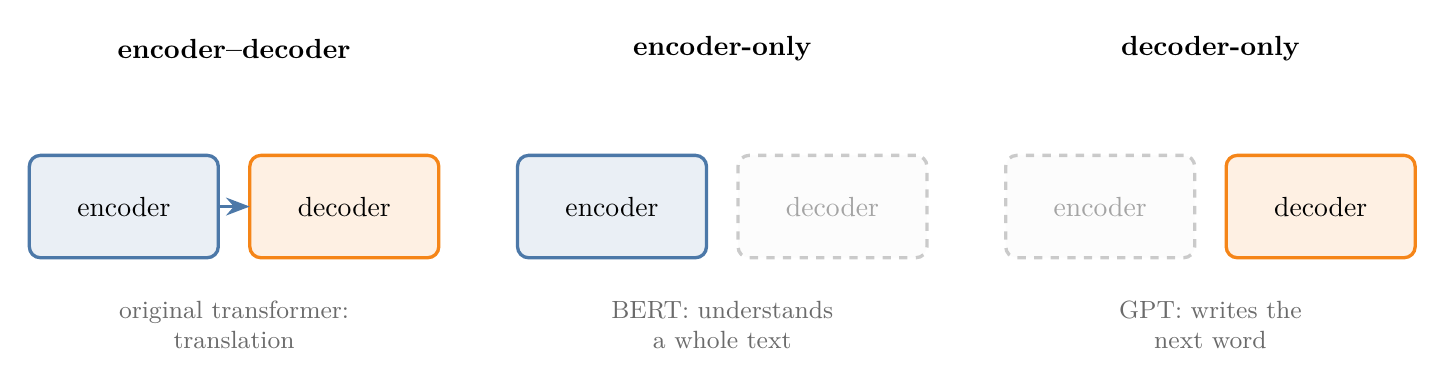
\begin{tikzpicture}[e/.style={box=cblue, minimum width=2.4cm, minimum height=1.3cm, font=\sffamily},
  d/.style={box=corange, minimum width=2.4cm, minimum height=1.3cm, font=\sffamily},
  off/.style={box=cgrey, minimum width=2.4cm, minimum height=1.3cm, font=\sffamily, draw opacity=0.35, fill opacity=0.15, text opacity=0.35, dashed}]
  \foreach \x/\t/\ex/\el/\dl in {0/{encoder–decoder}/{original transformer:\\translation}/e/d, 6.2/{encoder-only}/{BERT: understands\\a whole text}/e/off, 12.4/{decoder-only}/{GPT: writes the\\next word}/off/d} {
    \node[font=\sffamily\bfseries] at (\x+1.4,2.0) {\t};
    \node[\el] (en) at (\x,0) {encoder};
    \node[\dl] (de) at (\x+2.8,0) {decoder};
    \node[note] at (\x+1.4,-1.5) {\ex};
  }
  \draw[arrow, draw=cblue] (1.2,0) -- (1.6,0);
\end{tikzpicture}
\end{document}
